\chapter{Density-based size estimation}\label{sec:density}

Nodes in Swarm must utilise their full reserve capacity: nodes will potentially further replicate chunks in case they have unused reserve capacity beyond storing their share necessary for a system-wide level of redundancy required. To incentivise this, participating in the redistribution game involves a check called \emph{proof of resources} which is supposed to verify the size of reserve from which the reserve samples are generated.
The insight here is that the sample is the lowest range of a uniformly random variate over the entire 256-bit address space. Intuitively, the higher the original volume of the sampled set, the denser it is, the lower the expected maximum value in the sample.
Conversely, a constraint on the maximum value of the last element in the sample practically puts a minimum cardinality requirement on the sampled set using a solution called \emph{density based set size estimation}.

We are given $n$ independent, uniformly distributed values between 0
and 1.%
%
\footnote{Because we work with densities, the actual integer range is not relevant and results obtained for the unit interval can simply be rescaled to the Swarm use case by multiplying with $2^{256}$.}
%
Let the value of the $k$th smallest of these be $x_k$ (so the
smallest of the $n$ values is $x_1$, the second smallest is $x_2$,
and so on, up to $x_n$). What is the distribution of $x_k$, given
$n$? And what is the threshold value $u$ such that for any given
probability $\alpha$, the chance of obtaining an $x_k$ lower than
$u$ is $\alpha$?

Note that the distance between any two adjacent
values out of $n$ independent uniform variates follows an exponential
distribution, as long as $n$ is sufficiently large.% 
%
\footnote{This follows from
the fact that $n$ independent uniform variates can be thought of as realizing a Poisson process, whereby the timing of events is random, and
it is known that the nearest-neighbour distribution (i.e., waiting time
between two consecutive events) is then exponentially distributed.}
%
The rate parameter of this exponential distribution is $n+1$, where $n$
is increased by one to account for the fact that the expected gap
between adjacent values is $1/(n+1)$.%
%
\footnote{For $n=2$, the mean outcome
is $x_1 = 1/3$ and $x_2 = 2/3$; for $n = 3$, it is $x_1 = 1/4$,
$x_2 = 2/4$, $x_3 = 3/4$; and so on: for arbitrary $n$,
$x_i = i / (n+1)$, with the gap between adjacent values in this ideal
case always being $1/(n+1)$.}

We are after the distribution of the $k$th value,
%
\footnote{An alternative approach using order statistic  expresses $x_k$ via a beta distribution. It is very difficult to prove  that the Beta distribution's quantile function is a strictly decreasing function of $n$, which is a key piece of the argument presented here. Although this method is exact even for small $n$, in our case, $n$ always a very large number, therefore we adopted the other method.} 
%
$x_k$, which then
can be thought of as arising from the sum of $k$ independent
exponential variables, each with a rate parameter of $n+1$. This is
known to result in an Erlang distribution with shape parameter $k$ and
rate parameter $n+1$. Using $X(\lambda)$ to denote the exponential
distribution with rate $\lambda$ and $E(k,\lambda)$ to denote the
Erlang distribution with shape $k$ and rate $\lambda$:
\begin{equation}\protect\hypertarget{eq-exp-erlang}{}{
\sum_{i=1}^k X_i(n+1)
= E(k,n+1) ,
}\label{eq-exp-erlang}\end{equation} where the subscript $i$ in
$X_i(n+1)$ distinguishes between independent exponentially distributed
random variables. The probability density function $E(x, k,n+1)$ of
the Erlang distribution itself is given by
\begin{equation}\protect\hypertarget{eq-erlang-pdf}{}{
E(x, k, n+1)
= \frac{(n+1)^k x^{k-1} \text{e}^{-(n+1)x}}{(k-1)!} .
}\label{eq-erlang-pdf}\end{equation}

This distribution contains the answer to the first question: what is the
distribution of the $k$th smallest value out of $n$ independent
uniform variates between 0 and 1? For example, if $k=16$ and $n$ is
either 500, 750, or 1000, we get the distributions shown in
Figure~\ref{fig-erlang-example}.

\begin{figure}[!ht]
  \centering
  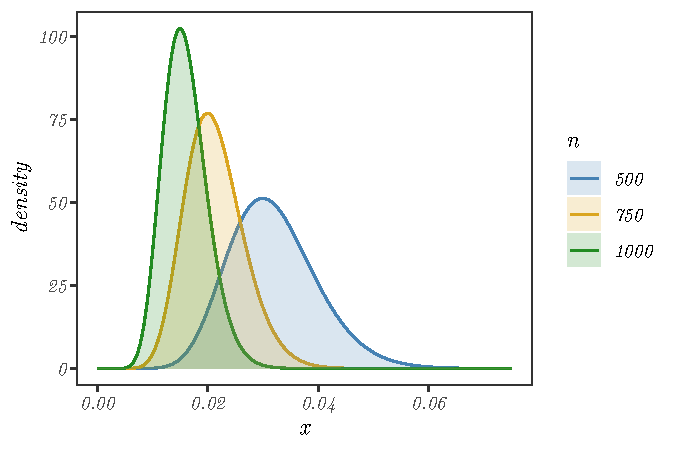
\includegraphics[width=.7\textwidth]{fig/fig-erlang-example-1.pdf}
  \caption[Probability density function of the Erlang distribution]{Probability density function $E(x, k, n+1)$ of the Erlang distribution, with $k=16$ and $n$ either 500, 750, or 1000.}
  \label{fig-erlang-example}
\end{figure}

We can now answer the second question: given $n$ and a confidence
level $\alpha$, what is the threshold value $u$ for $x_k$ such
that the probability that $x_k < u$ is equal to $\alpha$? That is,
we wish to know the value $x = u$ at which the probability
distribution has encompassed a given area of $\alpha$ (see figure~\ref{fig-alpha}).

\begin{figure}[!ht]
  \centering 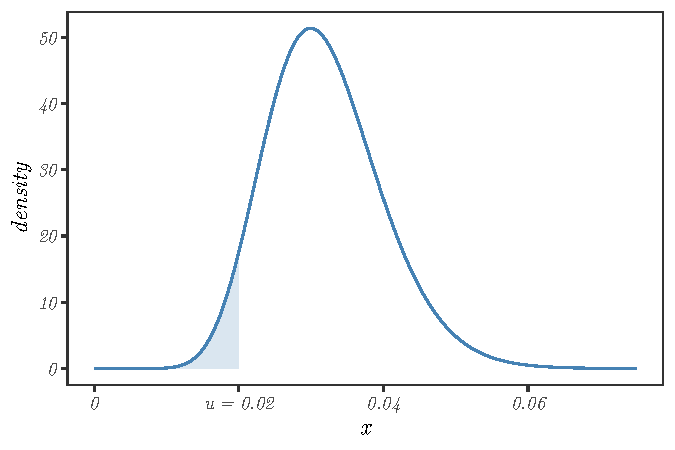
\includegraphics[width=.7\textwidth]{fig/fig-alpha-1.pdf}
  \caption[The 16th smallest value among $500$ random variates on unit interval]{The distribution of $x_{16}$, i.e., the 16th smallest value from among $n=500$ independently and uniformly drawn variates between 0 and 1. The area under the curve is shaded up to 5\% of its area. The point at which the shading stops is therefore the value $u$ for which there is only a 5\% chance of getting an even smaller $x_{16}$.}
  \label{fig-alpha}
\end{figure}

The area under
the curve of the Erlang distribution is given by its cumulative
distribution function $P(x,k,n+1)$, which is known to be
\begin{equation}\protect\hypertarget{eq-Erlang-cdf}{}{
P(x,k,n+1)
= \int_0^x E(y,k,n+1) \,\text{d}y
= \frac{1}{(k-1)!} \int_0^{(n+1)x} t^{k-1}\text{e}^{-t} \,\text{d} t .
}\label{eq-Erlang-cdf}\end{equation} The latter expression is sometimes
written as $\tilde{\gamma}(k,(n+1)x)$, where
\begin{equation}\protect\hypertarget{eq-gamma-regularized}{}{
\tilde{\gamma}(k,x)
= \frac{1}{\Gamma(k)} \int_0^x t^{k-1} \text{e}^{-t} \,\text{d}t
}\label{eq-gamma-regularized}\end{equation} is the regularized lower
incomplete gamma function. We therefore want to solve the equation
\begin{equation}\protect\hypertarget{eq-alpha}{}{
\alpha
= \int_0^u E(y,k,n+1) \,\text{d}y = P(u,k,n+1)
}\label{eq-alpha}\end{equation} for $u$.

Inverting this expression in $u$ (since the cumulative distribution
function increases monotonically in $u$, the inverse exists) leads to
the quantile function $Q(\alpha,k,n+1)$ of the Erlang distribution:
$u = Q(\alpha,k,n+1)$.
The quantile function is known to be expressible as
\begin{equation}\protect\hypertarget{eq-erlang-quantile}{}{
Q(\alpha,k,n+1)
= \frac{\tilde{\gamma}^{-1}(k,x)}{n+1} ,
}\label{eq-erlang-quantile}\end{equation} where
$\tilde{\gamma}^{-1}(k,x)$ is the inverse regularized lower incomplete
gamma function. Its particular form is of no interest to us, except for
two properties. First, it is positive for all $x$.%
%
\footnote{This stands to
reason: the quantile function of a distribution on
$x \in [0, \, \infty)$ is itself between 0 and $\infty$, and
$\tilde{\gamma}^{-1}(k,x)$ is just the quantile function of the Erlang
distribution times the positive constant $n+1$.}
%
Second, it is
independent of $n$. Instead, the entire dependence of
$Q(\alpha,k,n+1)$ on $n$ is given by the $n+1$ term in the
denominator of Equation~\ref{eq-erlang-quantile}. From this, we conclude
that $Q(\alpha,k,n+1)$ is a strictly decreasing function of $n$.

These two points lead to an important consequence. Say we compute the
threshold $u$ for a given $\alpha$ and $n$ in order to have an upper bound on a lower quantile. Now, if we were to
decrease $n$ but hold all other things equal, the threshold will
always get higher than what it was before. The threshold obtained for
higher values of $n$ may therefore serve as a conservative estimate of
the threshold for lower values: if $u$ is a threshold such that the
$k$th smallest out of $n$ uniform variates is only smaller than $u$ in
$\alpha$ of cases, then for any amount $m<n$, the chance of the
$k$th variate conforming to the same constraint (i.e., $x_k<u$) is now even smaller than $\alpha$. 

Conversely, if we were to constrain $x_k$ so that the probability of not getting a value smaller than $u$ is lower than $\beta$ (minimising a higher quantile), we find that the constraint remains true as $n$ is increased.

Armed with these results, let us see how
Equation~\ref{eq-erlang-quantile} can be used for the estimation
procedure.  
There are two problems to tackle, ultimately relating to the two aspects of a test's accuracy. First, we want to catch inadequate storers slacking on volume. In other words, we want to constrain the $x_k$ values so that we can safely say that any attacker with a stored volume below an acceptable size $n$ has a probability less than $\alpha$ to obtain such a small $x_k$ by pure chance. Construing the condition for $x_k<u$ as a test to filter honest players (just based on the size of their reserve), $1-\alpha$ expresses the \emph{sensitivity} of the test.
From the previous argument on the monotonic dependence of $\alpha$ on $n$, it is safe to use a condition that requires $x_k$ to stay below a threshold obtained for $n$. 

Second, we want to avoid situations when honest participants end up not satisfying the above constraint even though they sampled from a set larger than the required minimum. Given a target volume $m>n$, the error rate of false negatives is guaranteed to be less than $\beta$ obtained from the quantile function with parameters $m, k, \text{ and }u$. The quantity $1-\beta$ is the \emph{specificity} or \emph{precision}
of the test.



Figure~\ref{fig-ns} illustrates this
idea, for two different distributions in both the lower- and upper-end
estimation. What we want is to choose $u$ to simultaneously make sure
that dishonest players do not sneak through the system \emph{and} also that
honest players do not get excluded too often. This translates to make both $\alpha$
and $\beta$ as small as possible. 


\begin{figure}[!ht]
  \centering
  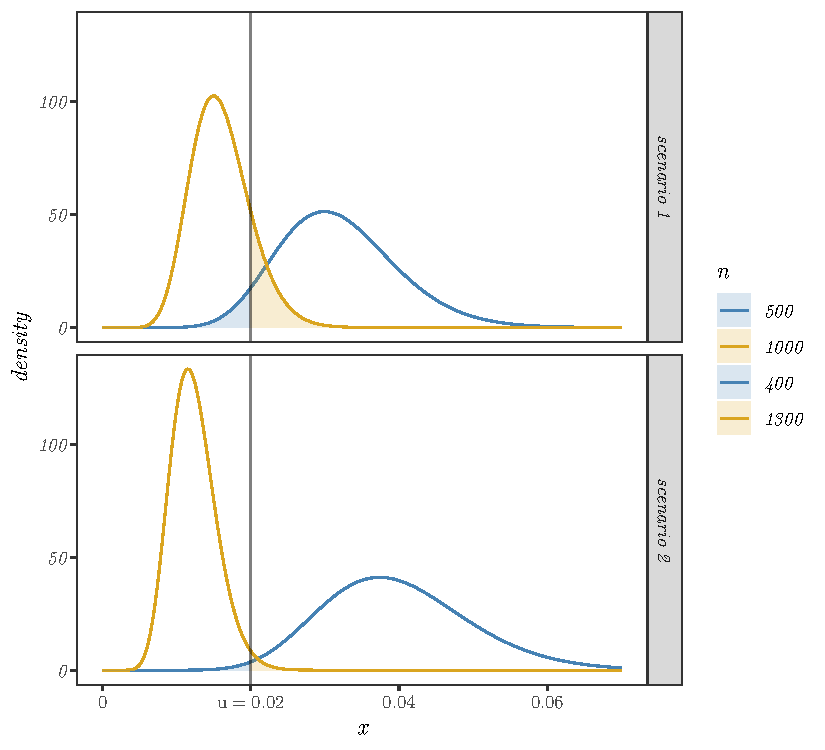
\includegraphics[width=.7\textwidth]{fig/fig-ns-1.pdf}
  \caption[Recall and precision of proof of reserve size validation]{Recall and precision of proof of reserve size validation: Any chosen $u$ will lead to different $\alpha$ and $\beta$ values, depending on $n$. Here $u$ is fixed at $0.02$. The top panel shows distributions for $x \equiv x_{16}$ with $n = 500$ (blue) and $n = 1000$ (yellow). The area left under the blue curve to the left of $u$ is equal to $\alpha$ (blue shade); the area under the yellow curve right of $u$ is equal to $\beta$ (yellow shade). If the curves overlap considerably (top), it is impossible to choose an $u$ such that $\alpha$ and $\beta$ are simultaneously small.}
  \label{fig-ns}
\end{figure}


One way to try and find the best compromise is by minimising
$\alpha + \beta$ (the \emph{accuracy} of the test) and pick the $u$ value at the optimum to be used in the proof of resources test. To this end, one
can vary $\alpha$ between 0 and 1 and, for each of its values, solve
the equation $\alpha = Q(1-\beta, k, n+1)$ (where $n$ is the larger
value, used for estimating $\beta$). This way, we get a $\beta$
value for every possible $\alpha$. Then, we can find the combination
which minimises $\alpha + \beta$, and determine the value of $u$
that leads to this optimum. As illustrated in
figure~\ref{fig-optim}, larger values of $k$ yield a trade-off curve along which
better accuracies can be achieved.

\begin{figure}[!ht]
  \centering
  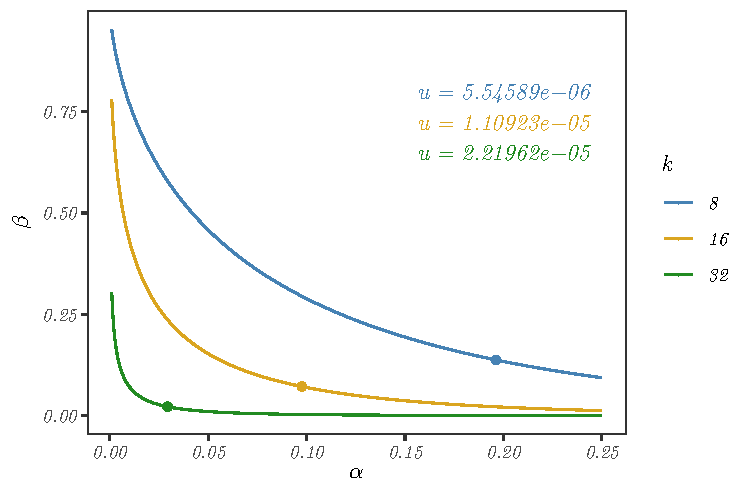
\includegraphics[width=.7\textwidth]{fig/fig-optim-1.pdf}
  \caption[Optimal accuracy of reserve size probe]{Optimal accuracy of reserve size probe By increasing $k$, one can get better optima for minimising $\alpha + \beta$. Here $n = 10^6$ for estimating $\alpha$ and $2\cdot 10^6$ for estimating $\beta$, and $k$ is either 8, 16, or 32 (colors). The values of $u$ associated with the optima are also shown.}
  \label{fig-optim}
\end{figure}



Table~\ref{tab:estim} summarizes the important numerical results in
Figure~\ref{fig-optim}.%
%
\footnote{Since the hash function used to generate random
variates does so in the range $[0, \, 2^{256}-1]$ instead of
$[0, \, 1]$, the calculated thresholds are scaled with $2^{256}$ to
show where they would fall in their actual range.}


\begin{table}[!ht]
 \centering
  \begin{tabular}{rrrrr}
  \toprule
  $k$ & $\alpha$ & $\beta$ & $u$ & $u \cdot 2^{256}$ \\
  \midrule
  8 & 0.196216 & 0.1373622 & $5.54589\cdot 10^{-6}$ & $6.421705\cdot 10^{71}$\\
  16 & 0.097612 & 0.0716570 & $1.10923\cdot 10^{-5}$ & $1.284401\cdot 10^{72}$\\
  32 & 0.029386 & 0.0219151 & $2.21962\cdot 10^{-5}$ & $2.570140\cdot 10^{72}$\\
  \bottomrule
  \end{tabular}
   \caption[Proof of density parameter calibration]{Proof of density parameter calibration. Assuming $n = 10^6$ and $m=2\cdot 10^6$ to calculate recall and precision error rates $\alpha$ and $\beta$, respectively, the cutoff value for the proof is calibrated by optimizing on acccuracy using sample sizes $8, 16, 32$.}
  \label{tab:estim}
\end{table}
